%!TEX root=../../autopilot.tex
\section{Sound Latency}
\label{sec:soundlatency}

\begin{margintable}[2cm]
\caption{Sound Latency Materials}
\label{tab:soundmaterials}
\noindent\begin{tabularx}{\linewidth}{lX}%
\toprule
\textbf{Sound Card} & \href{https://wiki.auto-pi-lot.com/index.php/HiFiBerry_Amp2}{Hifiberry Amp2} \\
\textbf{jack} & 1.9.22 \\
\textbf{Code} & \href{https://github.com/auto-pi-lot/plugin-paper/blob/main/plugin_paper/scripts/test_sound.py}{test\_sound.py} \\
\textbf{Replicate} & \texttt{python test\_sound.py} \\
\bottomrule
\end{tabularx}
\end{margintable}

We measured end to end, hardware input to sound output latency by measuring the delay between an external digital input and the onset of a 10kHz pure tone (Table \ref{tab:soundmaterials}). Sound playback was again triggered by the \texttt{Digital\_In} class's callback method, and sound samples were buffered in a \href{https://docs.python.org/3/library/collections.html#collections.deque}{deque} held in a separate process by the jack audio client between each trial. A \texttt{Digital\_Out} pin was wired to the \texttt{Digital\_In} pin in order to deliver the trigger pulse (but the \texttt{Digital\_Out} pin was uninvolved in the software trigger for sound output).

Autopilot's \href{http://jackaudio.org/}{jack} audio backend was configured with a \texttt{192kHz} sampling rate with a buffer with two periods of of \texttt{32} samples each for theoretical minimum latency of \texttt{0.33ms}\sidenote[][-2cm]{A previous version of this paper included benchmarking and comparison to Bpod and pyControl's sound onset latency, but since then both packages have changed substantially, including Bpod creating a new \href{https://sites.google.com/site/bpoddocumentation/assembling-bpod/hifi-module}{hifi sound module} based off HiFiBerry hardware very similar to the card used here, making those benchmarks obsolete. In this version we have omitted comparative benchmarks in favor of allowing the maintainers of those packages to publish their own benchmarks.}. We observed a median 1.35ms ($\pm$ 0.72 IQR) latency across 521 samples --- roughly 4x the theoretical minimum (Figure \ref{fig:lags}). This suggests that Autopilot eliminates most perceptible end-to-end latency, which is necessary for tasks that require realtime feedback. One clear future direction is to write the sound processing loop in a compiled language exposed with a foreign function interface (FFI) to decrease both latency and jitter.

\begin{figure}[hb!]
\caption{Autopilot has a median 1.35ms ($\pm$ .72 IQR) latency between an external trigger and sound onset. Individual trials (dots, n=521) are shown beneath a density plot (red area under curve) colored by quartile (shades, numbers above are median, first, and third quartile). This latency is roughly 4x the theoretical minimum (0.33ms, dashed line).}
\label{fig:lags}
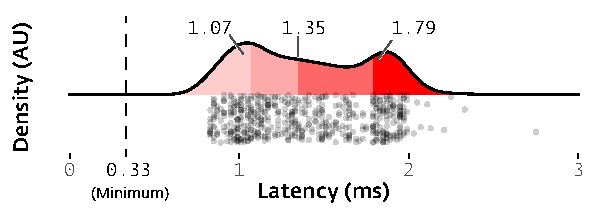
\includegraphics{figures/sound_latency.pdf}
\end{figure}